\chapter{Introduction}\label{introduction}
\quad\, Since the end of the 17th century, people have started to study the conversion of the energy into a useful form. The purpose was to utilise the available raw energy to produce works.\\

Denis Papin, a french person borned in 1647 in the region of Chitenay, developed one of the first conversion machine in 1690. The machine, a steam piston engine, was powered by steam which produced a back and forth movement of the piston head generating power.

\begin{figure}[h]
    \centering
    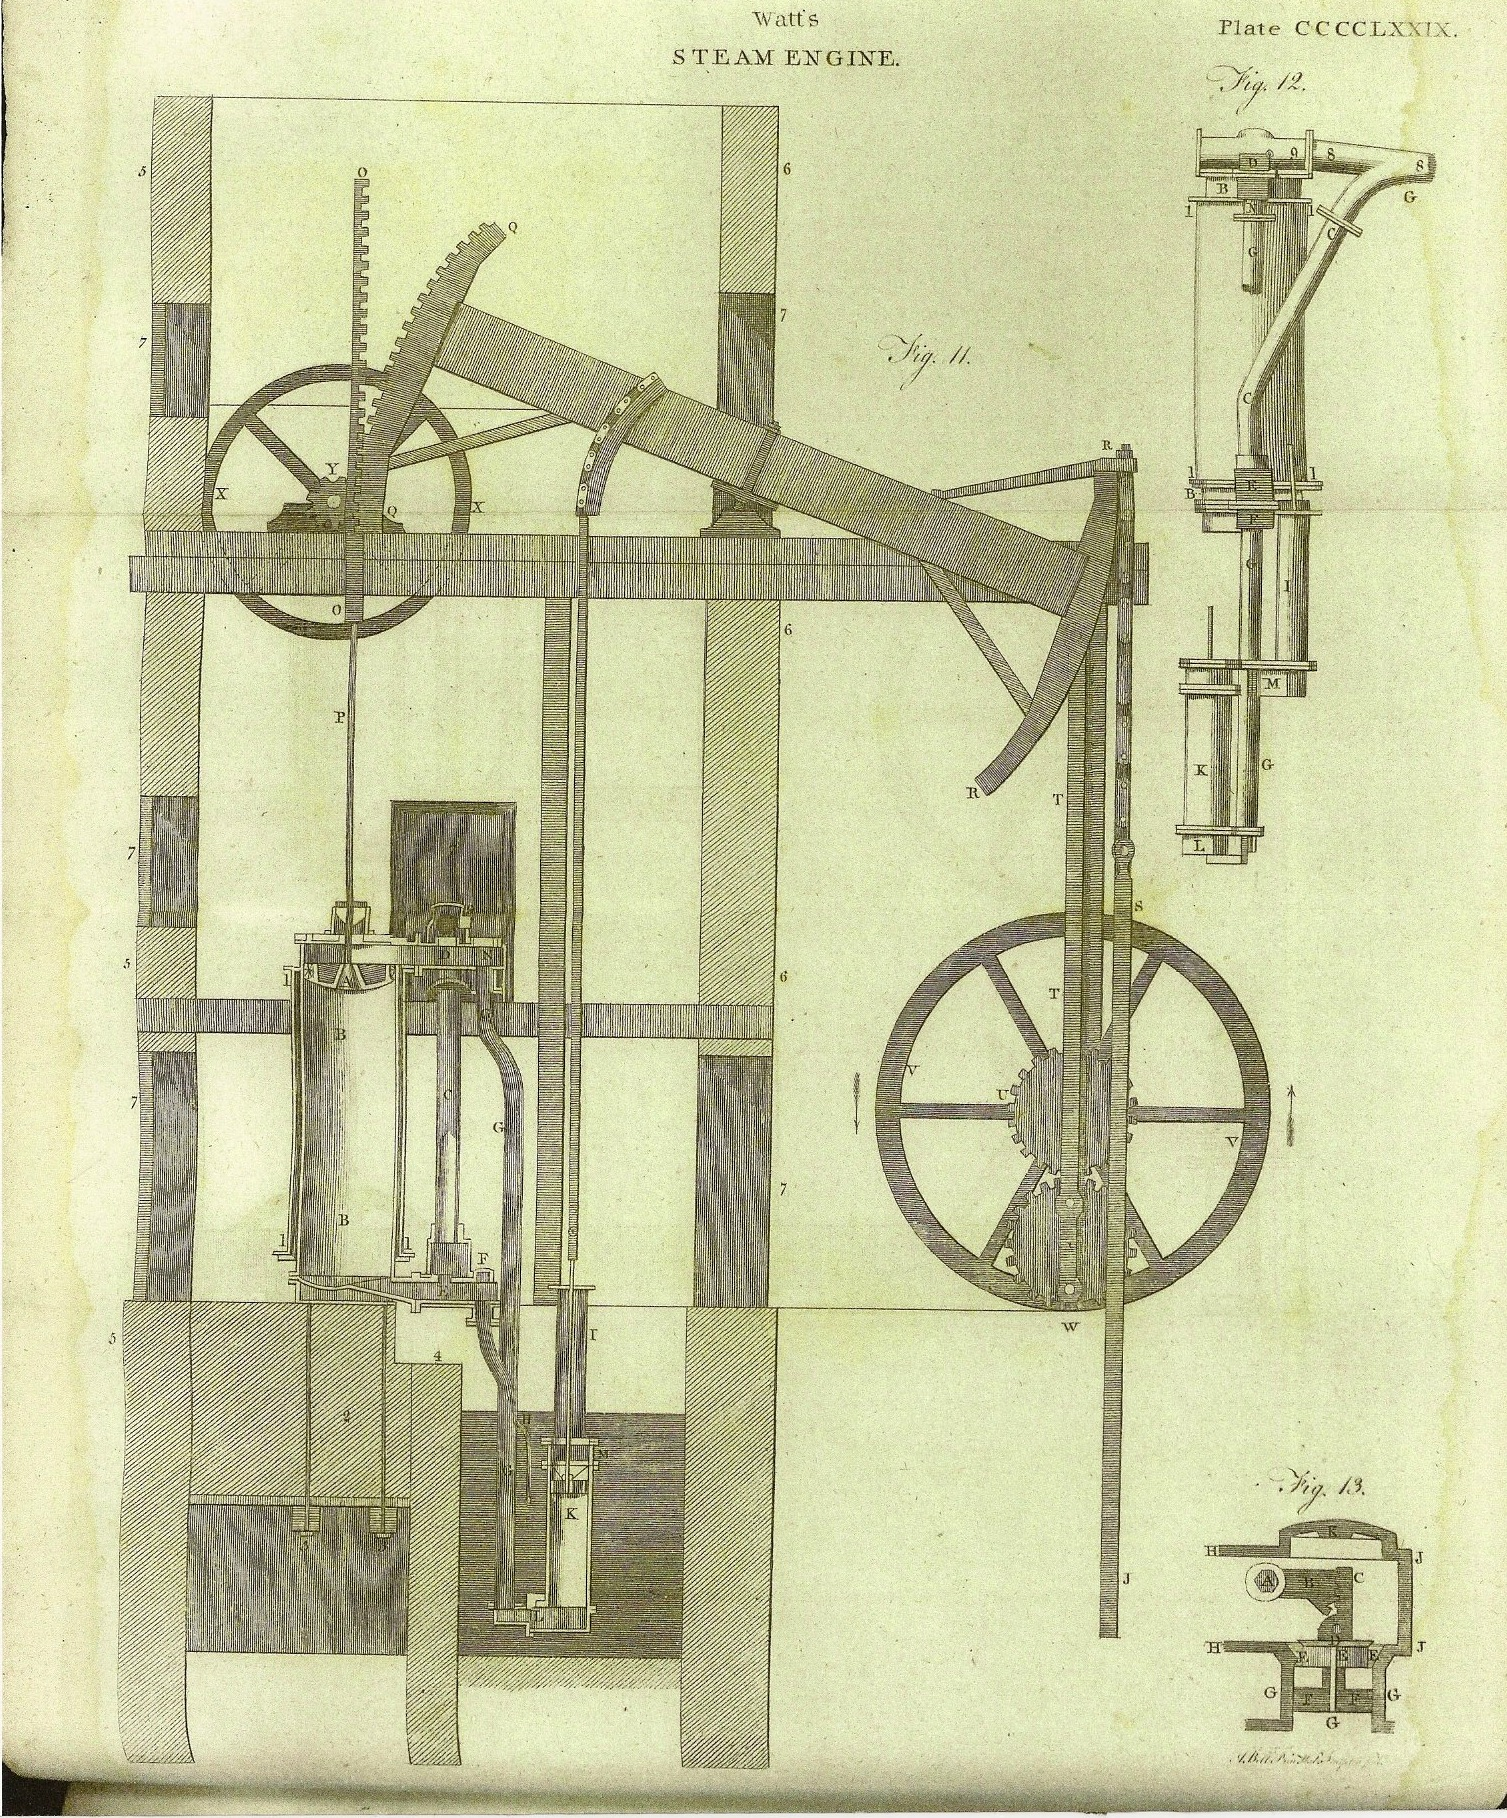
\includegraphics[width=0.5\textwidth]{Images/Introduction/WattsSteamEngine.jpeg}
    \caption{Watt steam machine\cite{Watt}}
    \label{fig:Watt}
\end{figure}

Then, later in the 18th, the British James Watt (1736 - 1819) invented and commercialised a steam machine. Thanks to the great marketing around his product, the machine (see Figure \ref{fig:Watt}), was very successful among the merchants. Indeed, it was sold as an alternative to horses and the capacity to produce works of the machine was express in horse power. 

James Watt named this quantifying unit the Watt unit (W), which will become later the standard unit for quantifying the power produced by a machine.\\

As a common knowledge, it is known that the steam machines have been an important element of the industrial revolution. The machines driven by wind and water have been progressively replaced by steam machines. It is only in the beginning of the 19th that this new technologies really started to be used. As examples, the applications were mining, merchandise transportation, etc...\\

In 1872, the American George Brayton (1830 - 1892) patented a gas internal combustion engine which was characterised by a continuous combustion\cite{Boles2006}. The  

% In the end of the $19^{\text{th}}$, the  American George Brayton (1830 - 1892) patented a gas internal combustion engine in 1872 which was characterised by a continuous combustion.\cite{Boles2006}. This was one of the first machine that was not utilising the steam as a media for work production.\\

% The Brayton's gas internal combustion engine was structurally comparable to a direct injection gasoline engine. 
% Today, the Brayton cycle is exclusively used in the gas turbine, where both the compressor and turbine are linked to the same shaft.\\
% Usually the cycle is open. This implies that the working fluid does not loop in the cycle but is instead constantly renew.\\
% The ideal Brayton cycle is characterised by the following 3 steps:
% \begin{enumerate}
%     \item Isentropic compression ($\mathbf{1} \Rightarrow\mathbf{2}$): The ambient air is compressed by the compressor. The consumed power during the compression is not negligible due to the large range of variation of the specific density of the gas. 
%     \item Constant pressure combustion ($\mathbf{2} \Rightarrow\mathbf{3}$): The compressed air enters the combustion chamber, along with the injected fuel. The resulting fumes has a much higher temperature. The pressure is assumed constant during the combustion.
%     \item Isentropic expansion ($\mathbf{3} \Rightarrow\mathbf{4}$): The hot fumes are expanded through the turbine to the ambient pressure. The expansion generate mechanical power that will partly used to feed the compressor. 
% \end{enumerate}

% The 3 steps are depicted on Figure \ref{fig:Open 
% Brayton}.\\


% \begin{figure}[h!]
%     \centering
%     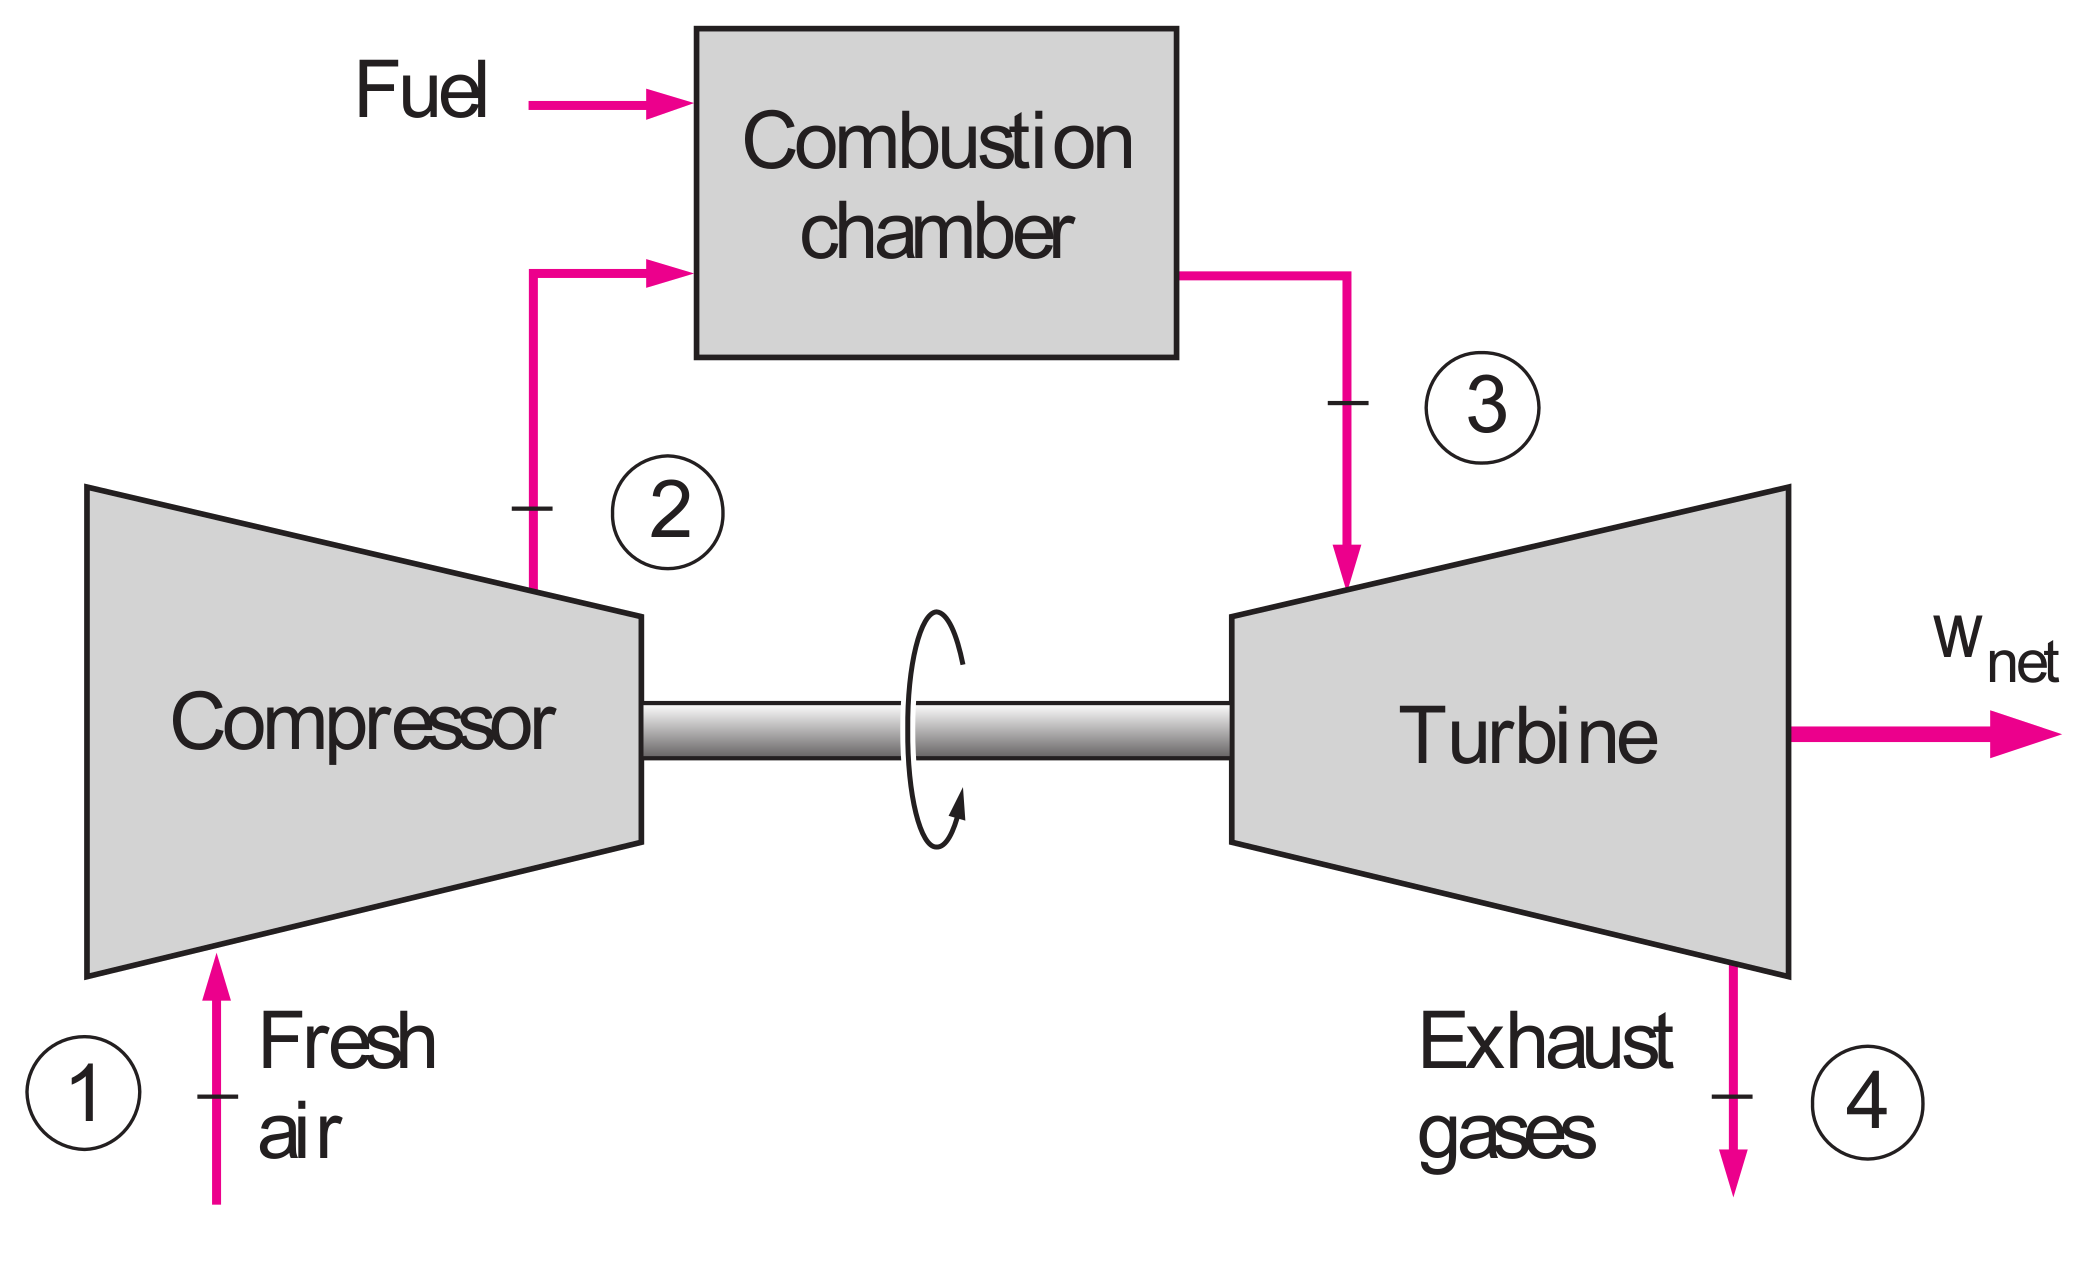
\includegraphics[width=0.8\textwidth]{Introduction/Open_Brayton_cycle.png}
%     \caption{Ideal open Brayton cycle \cite{Boles2006}}
%     \label{fig:Open Brayton}
% \end{figure}

% For the ideal Brayton cycle, it can be shown that the thermal efficiency\footnote{by definition, the thermal efficiency is given as the ratio between the net power output and the thermal power consumed.} is only an increasing function of the compression ratio $\Pi$.

% \begin{figure}[h!]
%     \centering
%     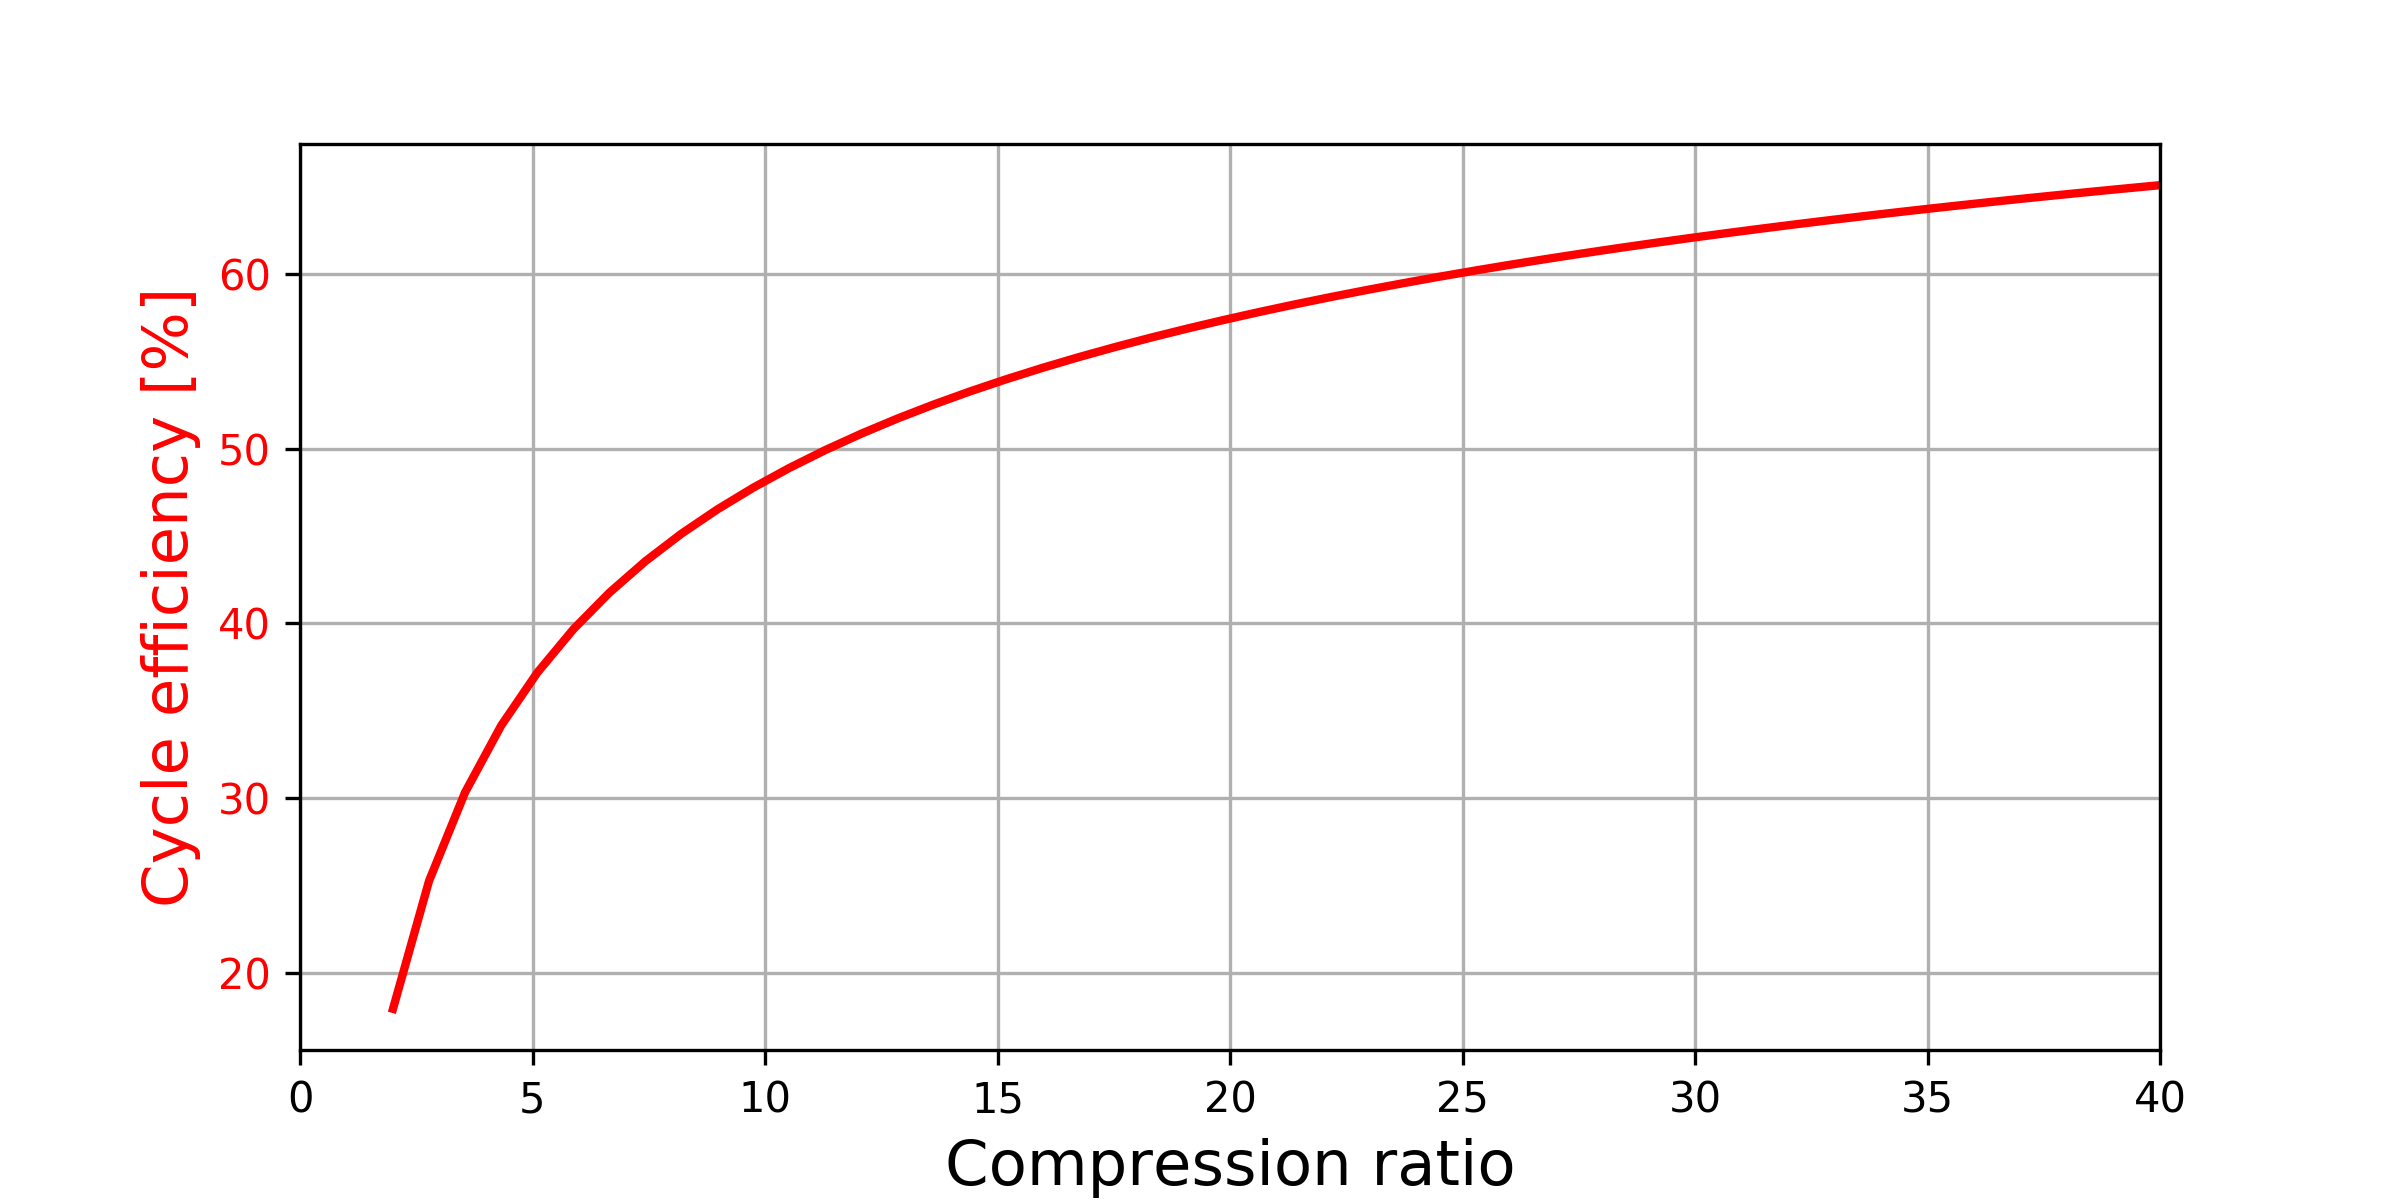
\includegraphics[width=0.8\textwidth]{Introduction/Efficiency_ideal_Brayton.png}
%     \caption{Efficiency as a function of the compression ratio (Ideal Brayton cycle)}
%     \label{fig:efficiency ideal Brayton}
% \end{figure}

% The mathematical expression (\ref{eq:efficiency_ideal_brayton})
%  of the efficiency is
%  \begin{equation}
%      \eta_{ideal} = 1 - \frac{1}{\Pi^\frac{\gamma-1}{\gamma}}\label{eq:efficiency_ideal_brayton}
%  \end{equation}
% with $\gamma = \frac{cp}{cv} > 0$ the heat capacity ratio.

% Typically, the $\gamma$ value is around 1.4. For this value, the graph \ref{fig:efficiency ideal Brayton} can be drawn. It can be seen that the cycle efficiency has an asymptotic value of 100\% that will be reached for an infinite compression ratio.\\

% There exists a variant of the Brayton cycle which is closed and recirculates the working fluid during operation.

% For this configuration, a heat source heat up the working fluid before entering the turbine. Then, a second heat-exchanger is insert between the outlet of the turbine and the inlet of the compressor to cool down the working fluid.\\

% A schematic of the closed Brayton cycle is drawn on Figure \ref{fig:Closed Brayton}.

% \begin{figure}[h!]
%     \centering
%     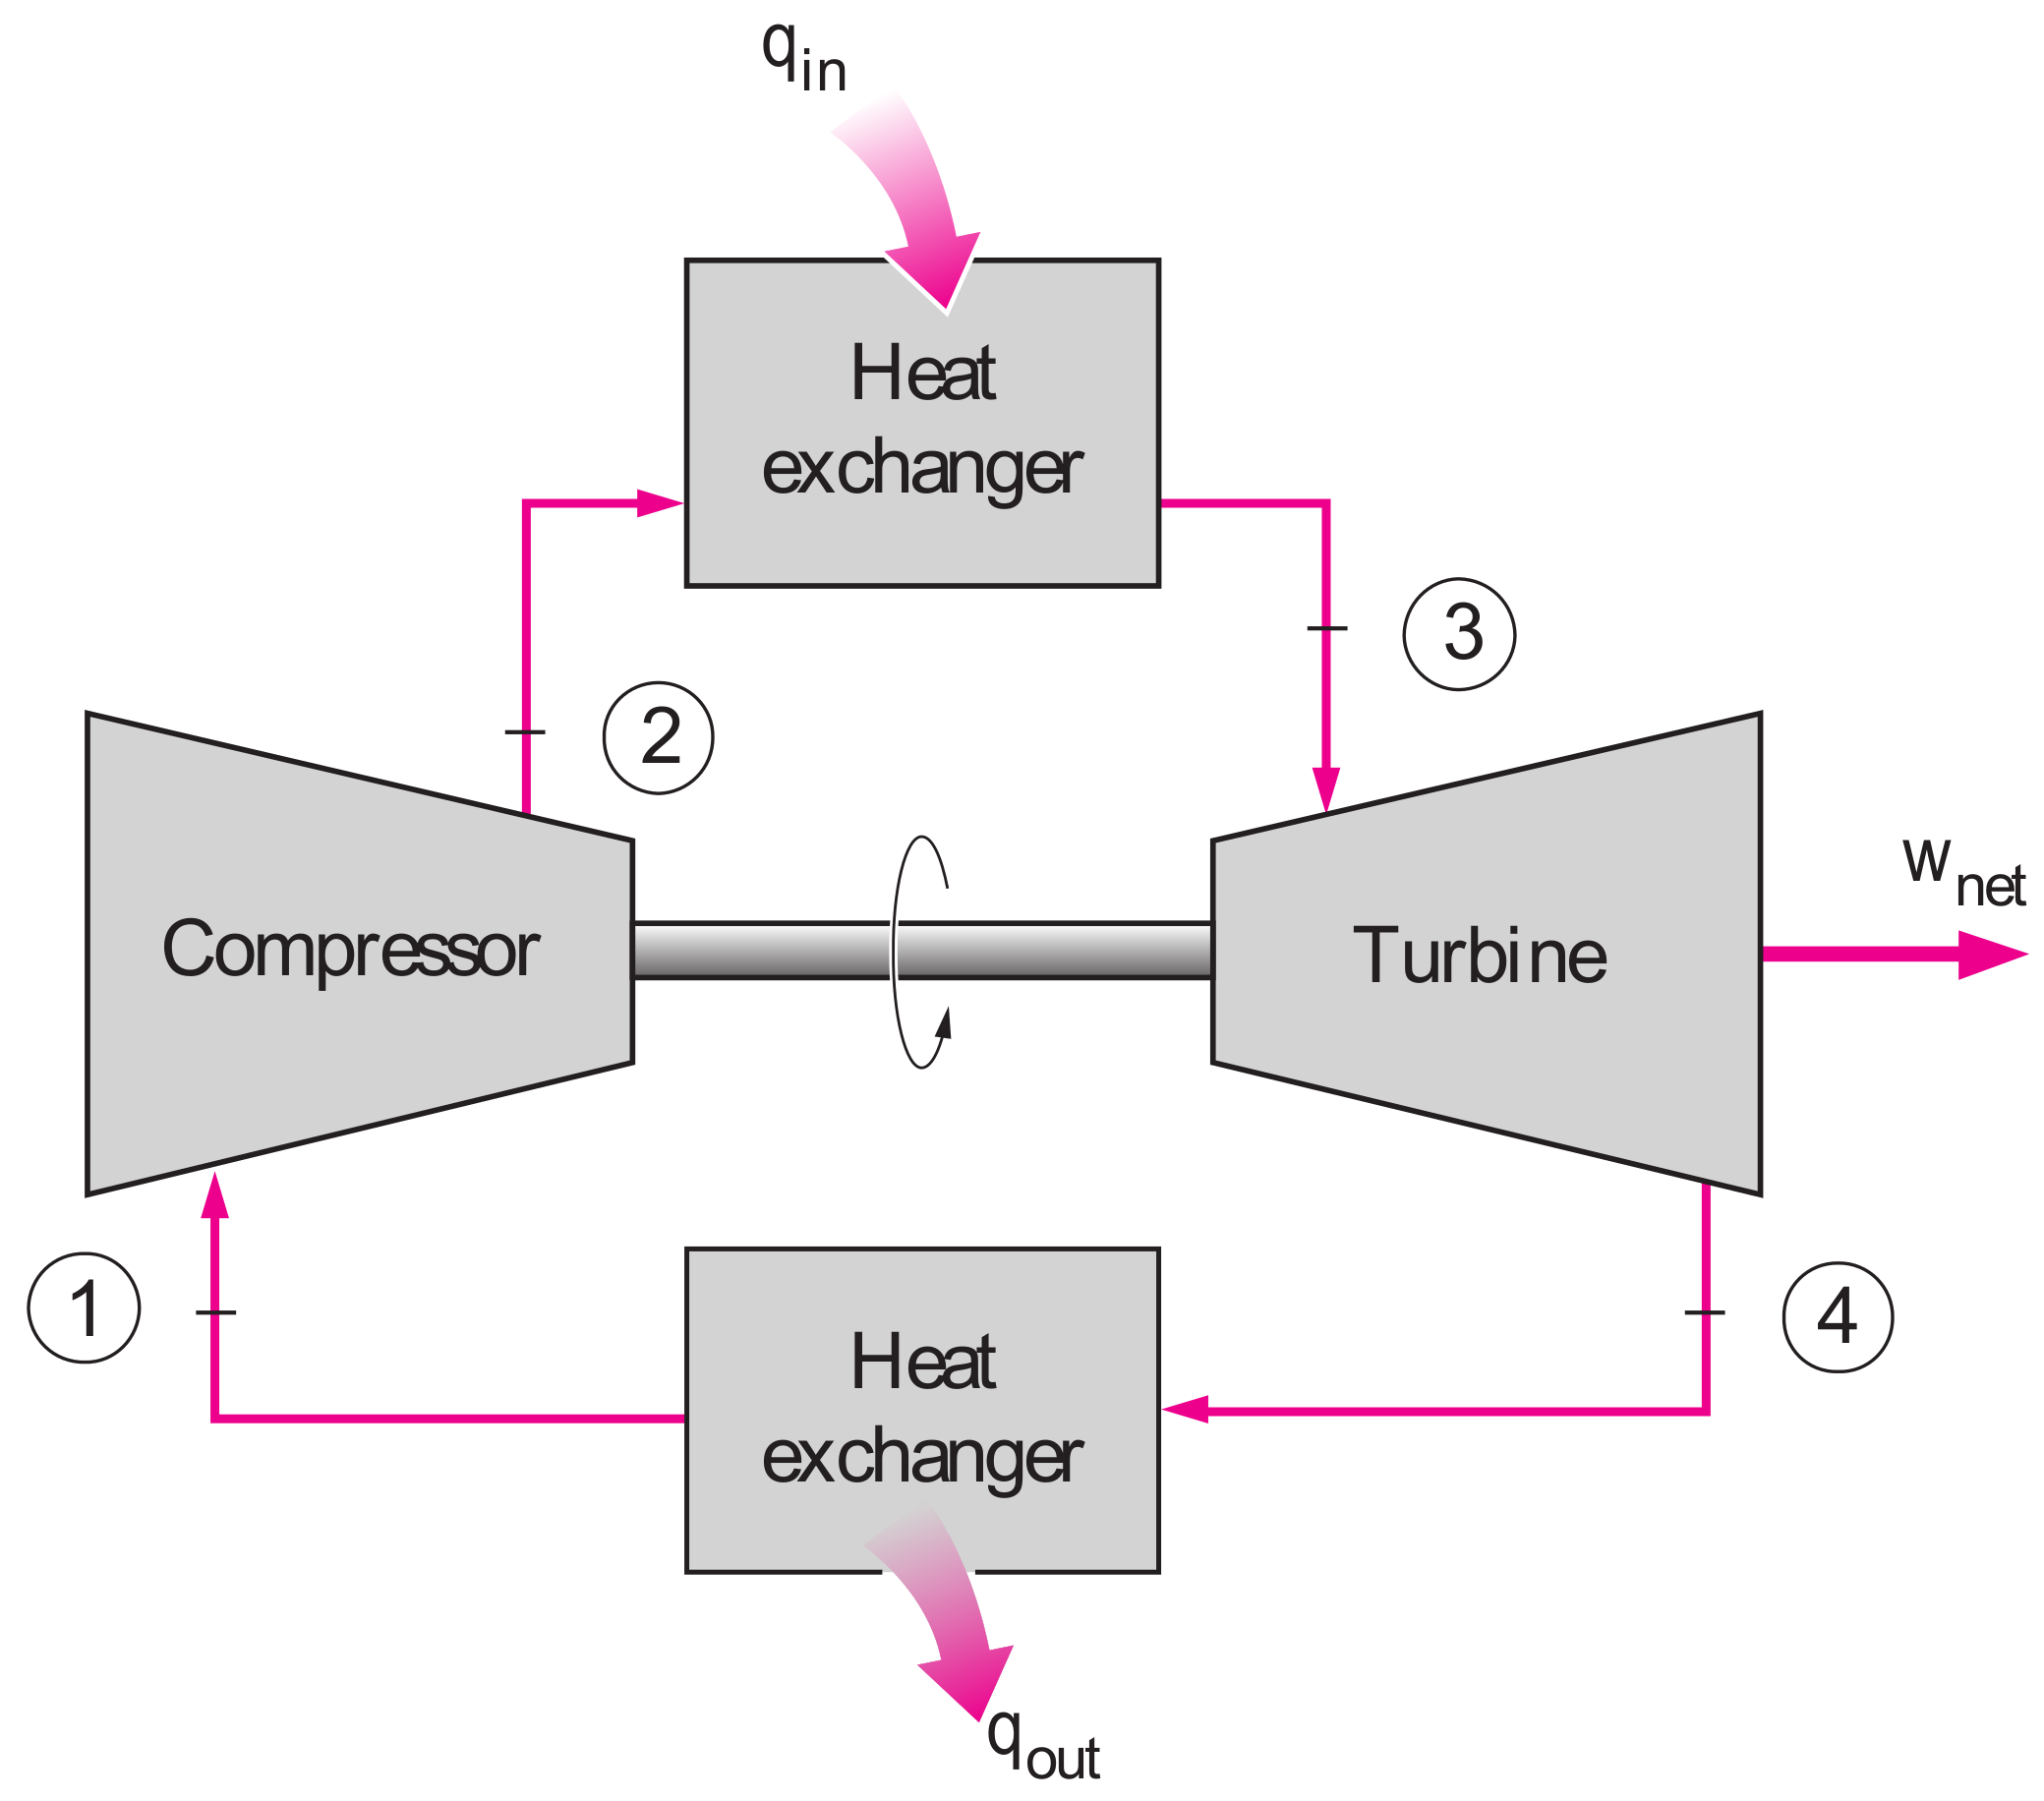
\includegraphics[width=0.8\textwidth]{Introduction/Closed_Brayton_cycle.png}
%     \caption{Ideal closed Brayton cycle \cite{Boles2006}}
%     \label{fig:Closed Brayton}
% \end{figure}

% The closed Brayton cycle often operates using super critical carbon dioxide (sCO2) as working fluid. These sCO2 cycles combine the advantages of the open Brayton cycle and of the Rankine (steam) cycle.

% Indeed, it can be shown that after the heat rejection process (step (1) on Figure \ref{fig:Closed Brayton}, the density of the gas is quite high. This high density will reduce the work done by the compressor in comparison with the open Brayton cycle.\cite{2017}.
% For the same reason, the size turbine of the sCO2 cycle can be decreased compared to the Rankine cycle.\\

% In this work, only the open Brayton cycle will be studied. Therefore, the prefix \textit{open} and \textit{closed} will be dropped to lighten the writing.

% \section{Improvements of the ideal Brayton cycle}
% \quad\; From the initial ideal Brayton cycle, several modification can be done to improve the thermal efficiency of the system.\\
% This section will be dedicated to the discussion about the possibility of improvement and those benefits to the system.

% \subsection{Reduction of exhaust gas temperature}
% The first improvement will be focused on the reduction of the temperature of the gas when ejected to the atmosphere. Indeed, there still remains useful heats in the exhaust gas.

% By introducing a heat-exchanger (called regenerator) that will pre-heat the air at the inlet of the combustion chamber, the hot gas will be cooled down from 800\degree C to around 300\degree C\footnote{those are order of magnitude}. This is illustrated on Figure \ref{fig:Brayton w/ regenerator}.

% \begin{figure}[h!]
%     \centering
%     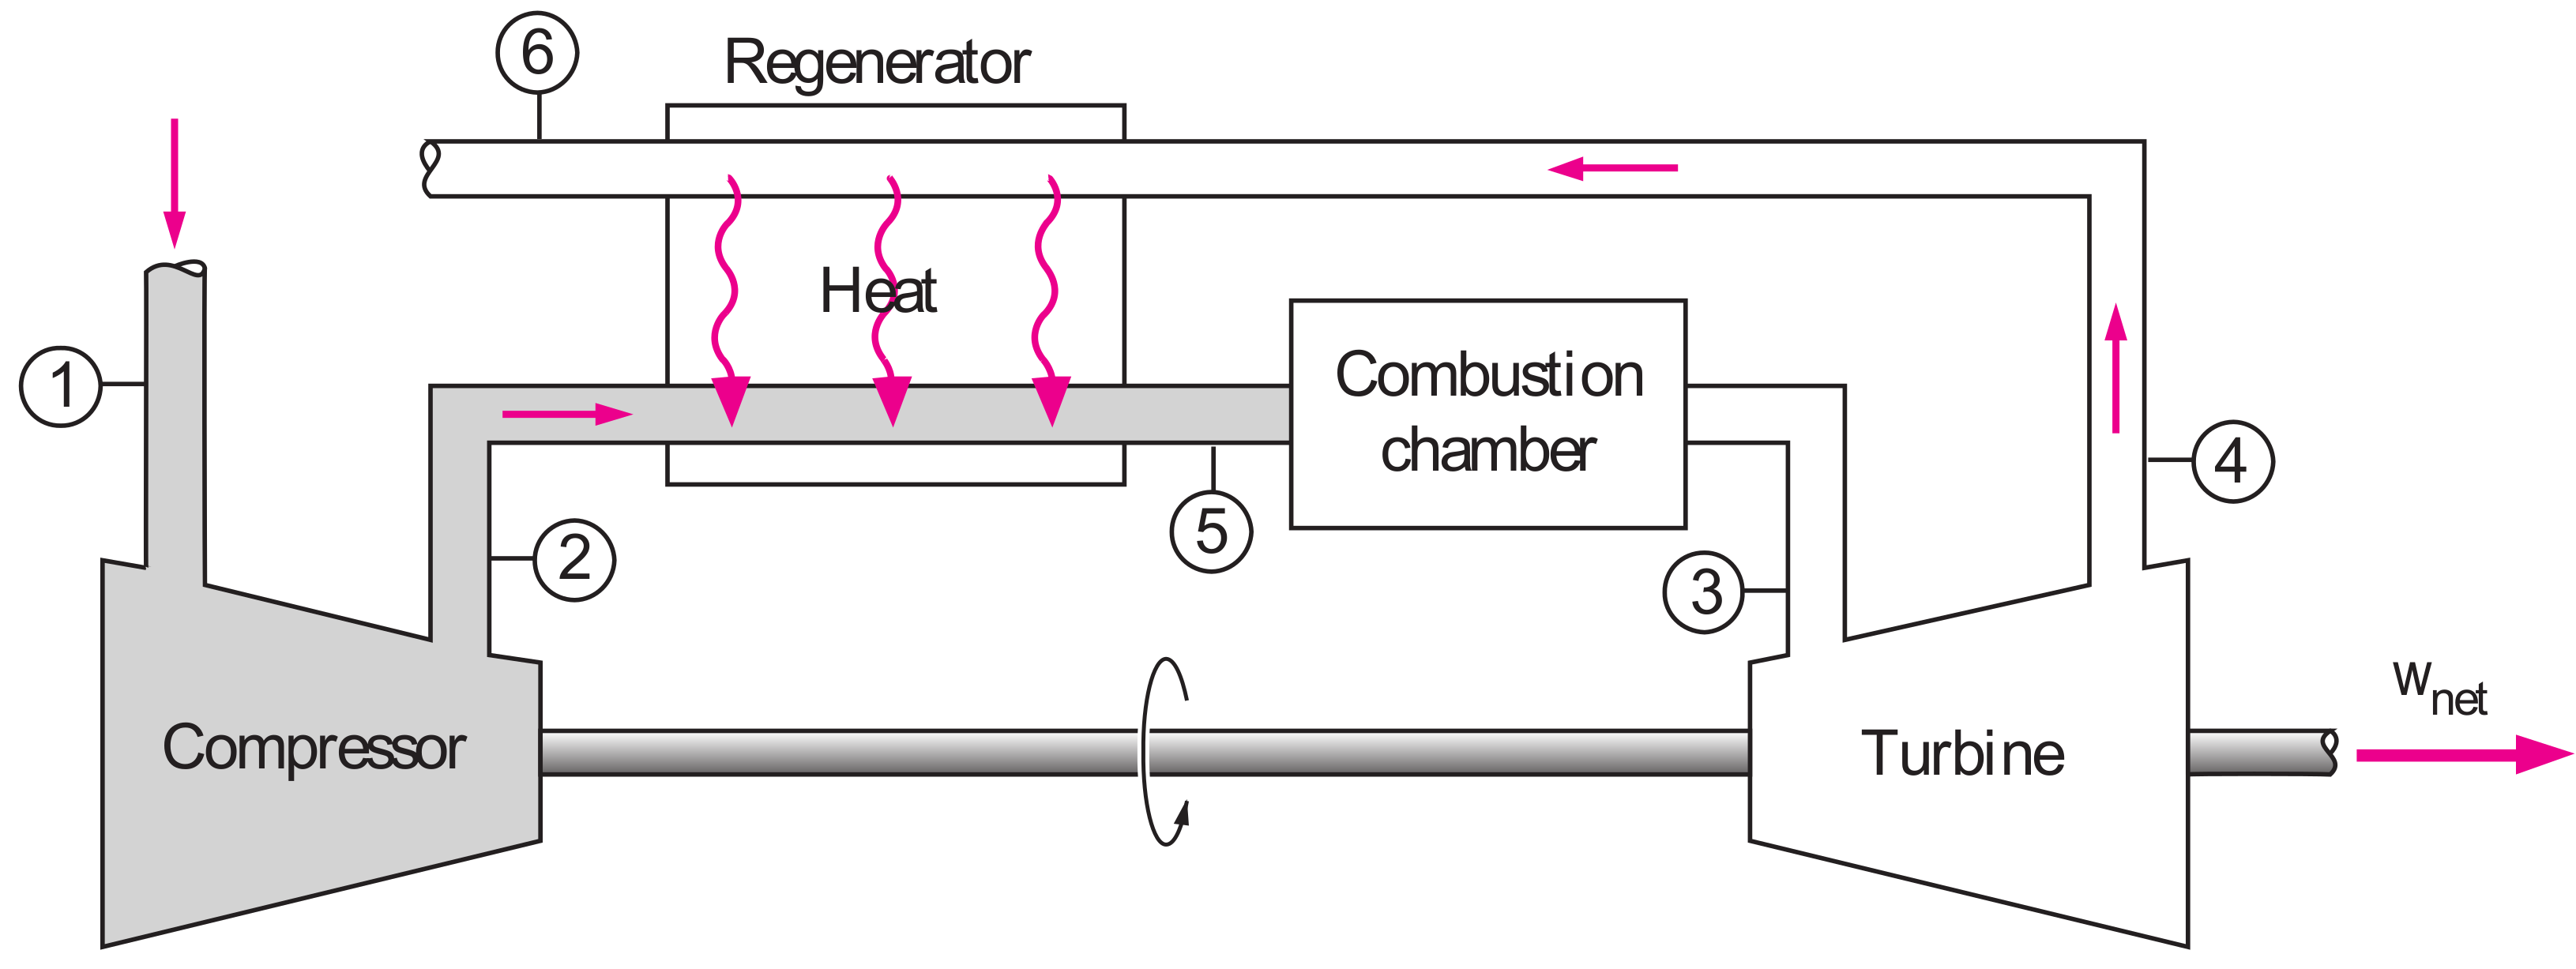
\includegraphics[width=0.8\textwidth]{Introduction/Regen_Brayton_cycle.png}
%     \caption{Ideal Brayton cycle with regenerator \cite{Boles2006}}
%     \label{fig:Brayton w/ regenerator}
% \end{figure}

% There, it can be shown that the efficiency is an increasing function of the turbine inlet temperature (TIT) and a decreasing function of the compression ratio ($\Pi$). It is expressed in the relation (\ref{eq:efficiency_ideal_regen_Brayton}).
% \begin{equation}
%     \eta_{ideal, regen} = 1 - \frac{T_1}{T_3}\Pi^\frac{\gamma-1}{\gamma}\label{eq:efficiency_ideal_regen_Brayton}
% \end{equation}
% where $T_1$ is the inlet temperature of the air and $T_3$ is the TIT.\\

% For a given TIT, it can be noticed that there is a given pressure ratio such that beyond, the regenerator deteriorate the cycle efficiency. The Figure \ref{fig:efficiency ideal Brayton w/ and w/o regenerator} illustrates this statement.

% Thus, for small and medium plants where the pressure ratio is not too big, regenerator will often be added considering the huge gain for the efficiency.

% \begin{figure}[h!]
%     \centering
%     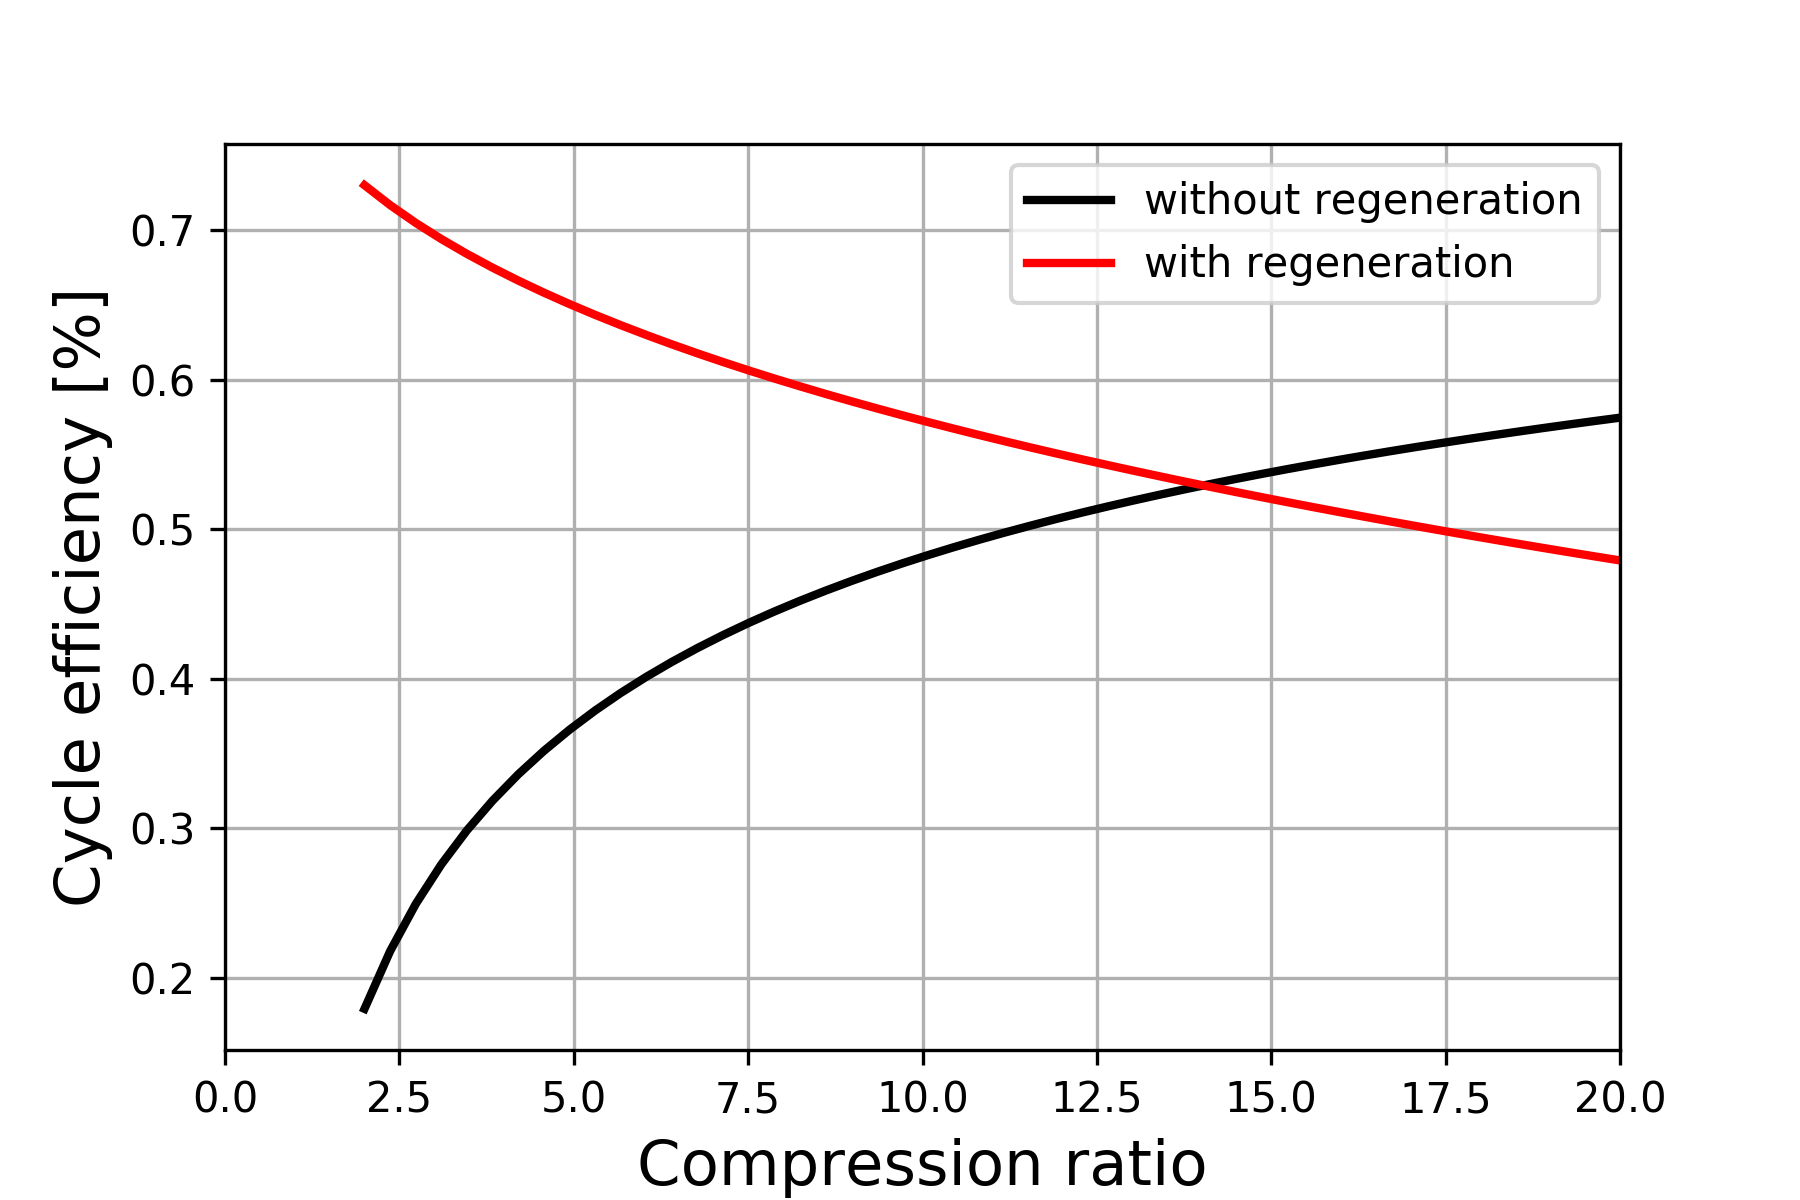
\includegraphics[width=0.8\textwidth]{Introduction/Efficiency_ideal_Brayton_regen.png}
%     \caption{Efficiency as a function of the compression ratio with a turbine inlet temperature (TIT) of 1300K (Ideal Brayton cycle with and without regenerator)}
%     \label{fig:efficiency ideal Brayton w/ and w/o regenerator}
% \end{figure}

% At the exit of the regenerator, there still have some remaining heat in the gas. This heat can be used ether to heat up water for cogenerator or, it can drive a second cycle that will utilise it as hot heat source.
% \section{Optimisation of the compression and expansion}

% An alternative exists to improve the efficiency of the cycle. By decreasing (resp. increasing) the compression power consumption (resp. the turbine power output), the efficiency will likely increase. It is done by splitting the compression and the expansion into multiple intermediate stages.

% Between each stage the fluid is taken back to its initial level of temperature using an intercooler or a reheater, respectively for the compression and the expansion unit.

% Often, the number of stages are identical for the compression unit and the expansion unit. A two-stages gas cycle with regenerator is illustrated on Figure \ref{fig: multistage}.\newpage

% \begin{figure}[h!]
%     \centering
%     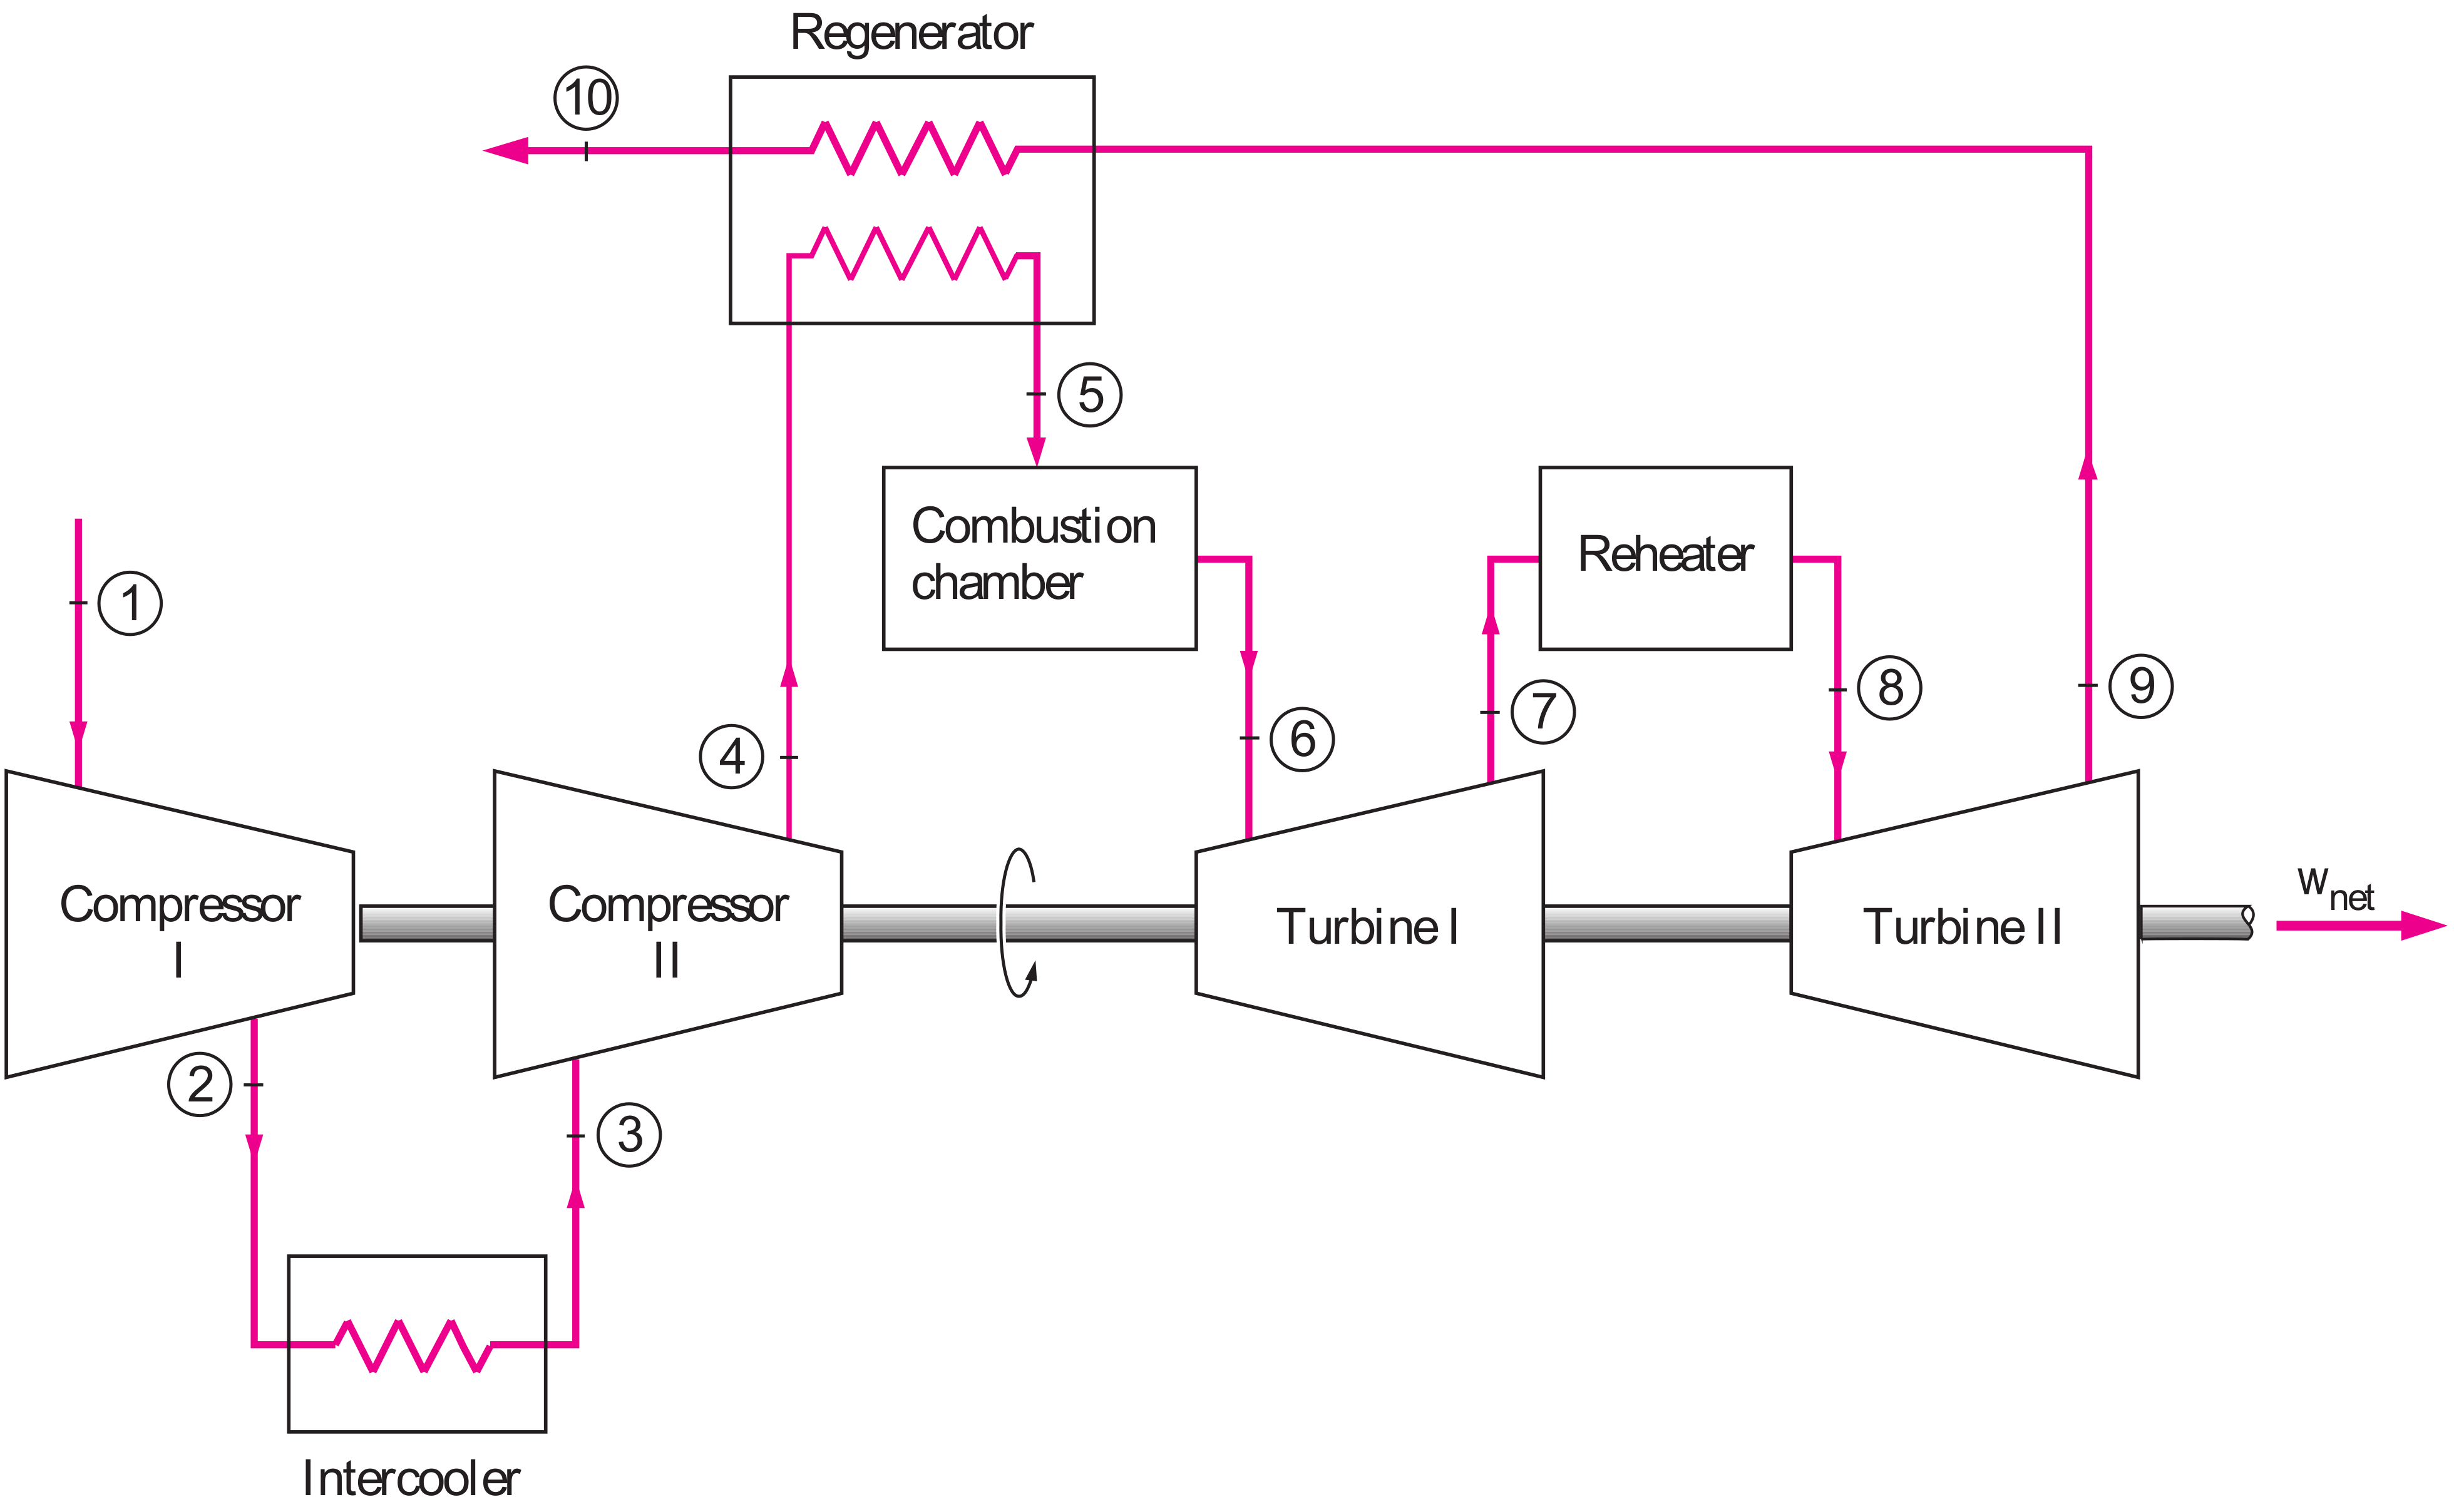
\includegraphics[width=0.8\textwidth]{Introduction/Brayton_cycle_multi.png}
%     \caption{Two-stage Brayton cycle with regenerator\cite{Boles2006}}
%     \label{fig: multistage}
% \end{figure}
 
% As the number of stages increases, the temperature variation during the compression and expansion phases becomes less pronounced. It can be shown that for an infinite number of stages, these transformations become isothermal and the cycle efficiency is equal to the Carnot efficiency. This trend is depicted on Figure \ref{fig:efficiency multistage}.

% \begin{figure}[h!]
%     \centering
%     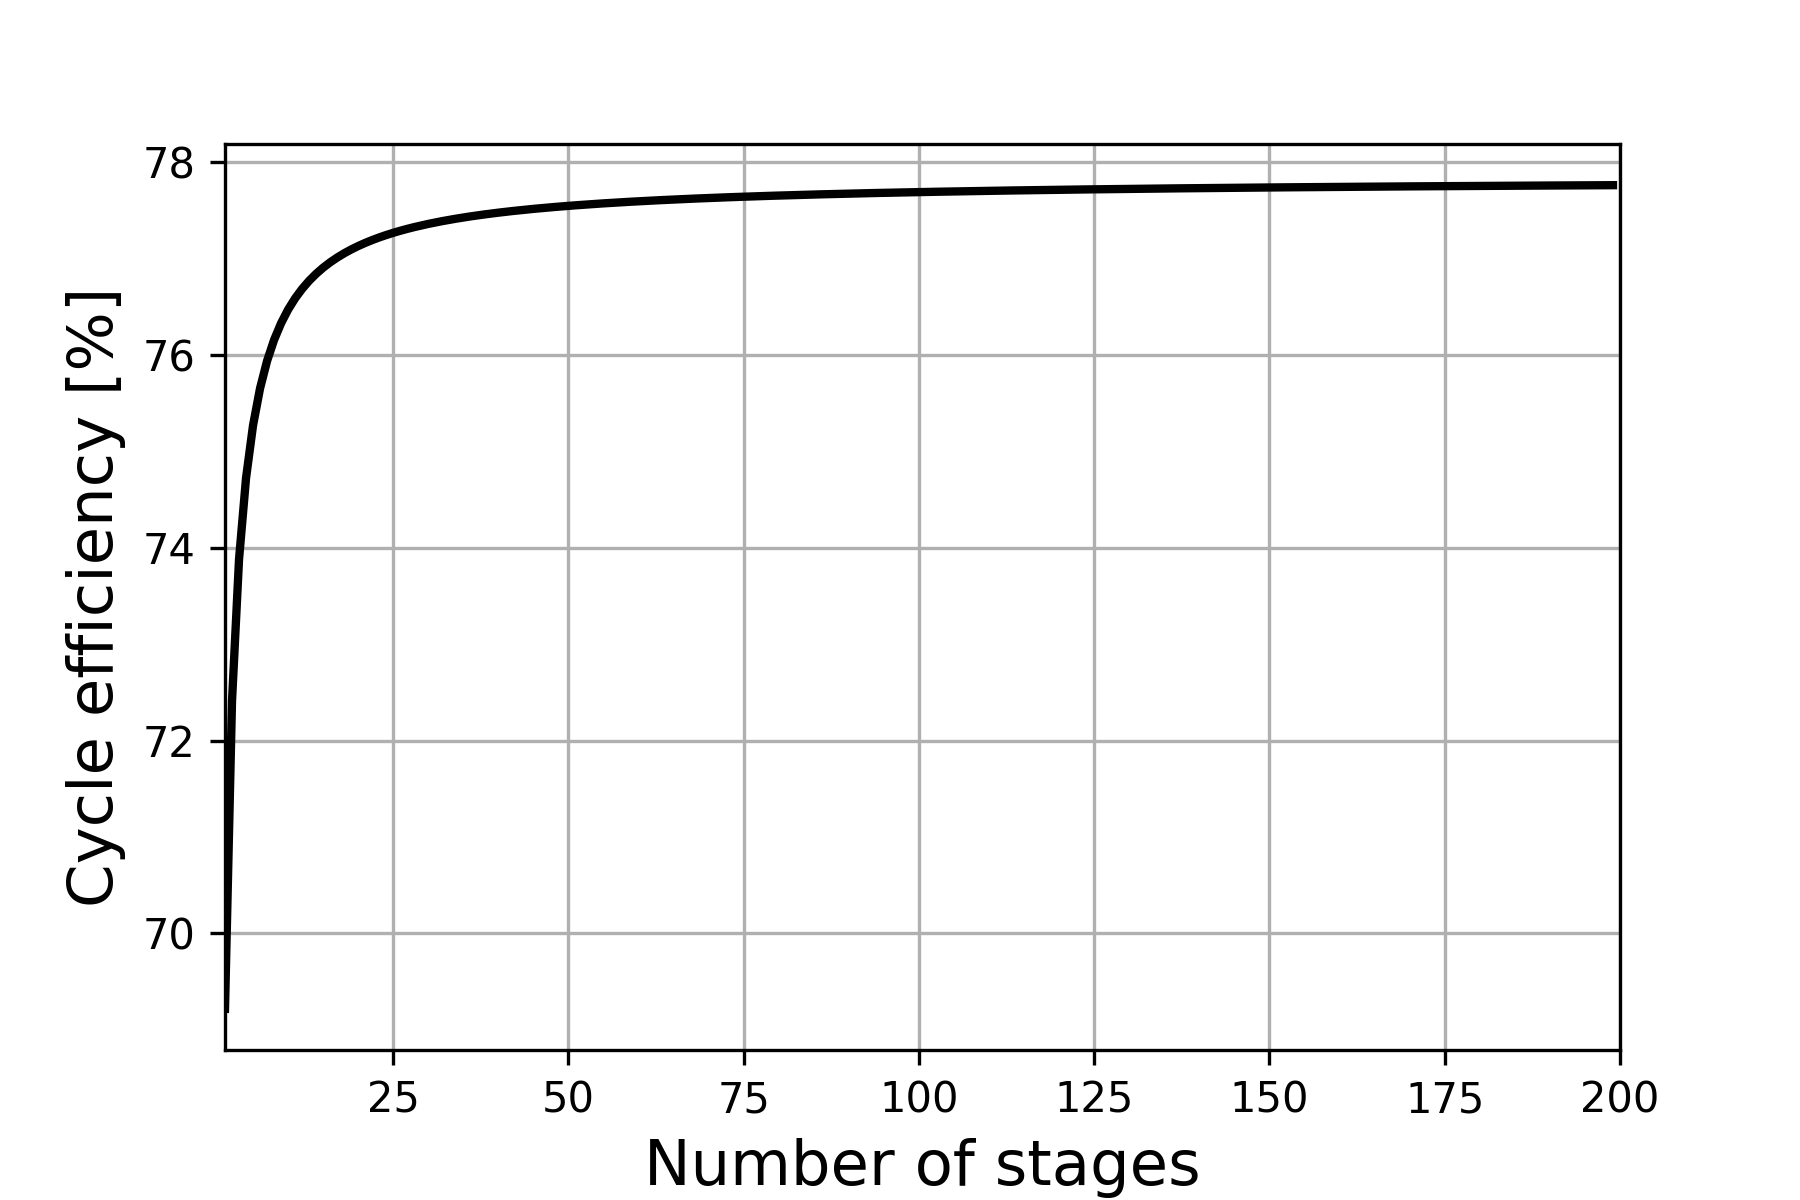
\includegraphics[width=0.8\textwidth]{Introduction/Efficiency_staged_Brayton.png}
%     \caption{Efficiency as a function of the number of stages (Staged Brayton cycle)}
%     \label{fig:efficiency multistage}
% \end{figure}

% \section{Focus on the non-ideal case}
% From now, it has been supposed that all the components were ideal. For the compressor and the turbine, this meant that the compression and expansion were performed without irreversibility. For the 
